%%%%%%%%%%%%%%%%%%%%%%%%%%%%%%%%%%%%%%%%%%%%%%%%%%%%%%%%%%
\frame {\frametitle{The Spark Shuffle Mechanism}
%%%%%%%%%%%%%%%%%%%%%%%%%%%%%%%%%%%%%%%%%%%%%%%%%%%%%%%%%%
\begin{itemize}
	\item {\bf Same concept as for Hadoop MapReduce, involving:}
	\begin{itemize}
		\item Storage of ``intermediate'' results on the local file-system
		\item Partitioning of ``intermediate'' data
		\item Serialization / De-serialization
		\item Pulling data over the network
	\end{itemize}

	\vspace{20pt}

	\item {\bf Transformations requiring a shuffle phase}
	\begin{itemize}
		\item \texttt{groupByKey()}, \texttt{reduceByKey()}, \texttt{sortByKey()}, \texttt{distinct()}
	\end{itemize}

	\vspace{20pt}

	\item {\bf Various types of Shuffle}
	\begin{itemize}
		\item \emph{Hash Shuffle}
		\item \emph{Consolidate Hash Shuffle}
		\item \emph{Sort-based Shuffle}
	\end{itemize}
\end{itemize}
}

%%%%%%%%%%%%%%%%%%%%%%%%%%%%%%%%%%%%%%%%%%%%%%%%%%%%%%%%%%
\frame {\frametitle{The Spark Shuffle Mechanism: an Illustration}
%%%%%%%%%%%%%%%%%%%%%%%%%%%%%%%%%%%%%%%%%%%%%%%%%%%%%%%%%%
\begin{figure}[h]
  \centering
  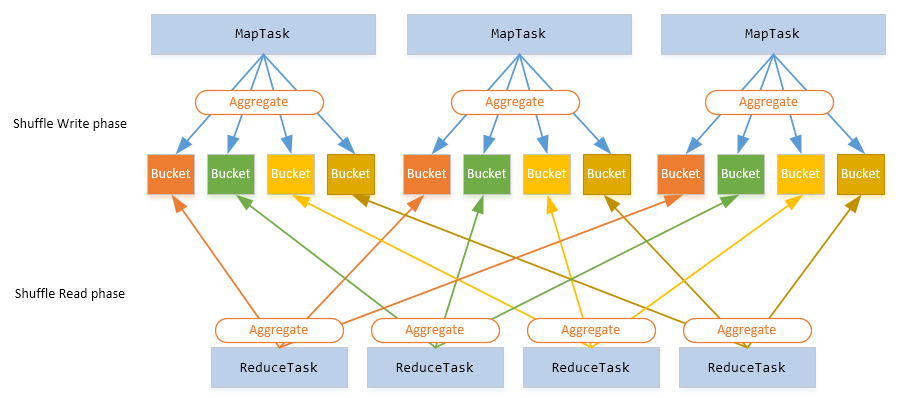
\includegraphics[scale=0.35]{./Figures/spark_shuffle}
  \label{fig:spark_shuffle}
\end{figure}

\begin{itemize}
	\item {\bf Data Aggregation}
	\begin{itemize}
		\item Defined on \texttt{ShuffleMapTask}
		\item Two methods available:
		\begin{itemize}
			\item \texttt{AppendOnlyMap}: in-memory hash table combiner
			\item \texttt{ExternalAppendOnlyMap}: memory + disk hash table combiner
		\end{itemize}
	\end{itemize}
	\item {\bf Batching disk writes to increase throughput}
\end{itemize}
}

%%%%%%%%%%%%%%%%%%%%%%%%%%%%%%%%%%%%%%%%%%%%%%%%%%%%%%%%%%
\frame {\frametitle{The Spark Shuffle Mechanism: Implementation Details}
%%%%%%%%%%%%%%%%%%%%%%%%%%%%%%%%%%%%%%%%%%%%%%%%%%%%%%%%%%
\begin{figure}[h]
  \centering
  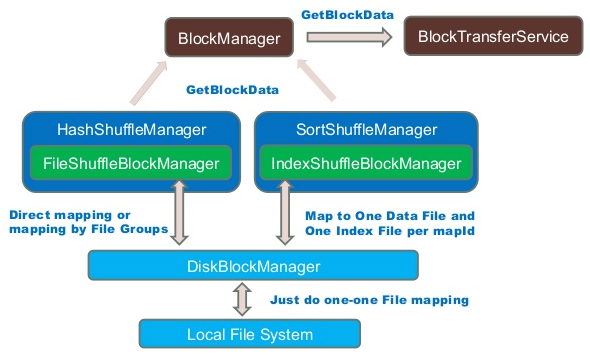
\includegraphics[scale=0.33]{./Figures/shuffle_diagram}
  \label{fig:spark_shuffle_diagram}
\end{figure}

\begin{itemize}
	\item {\bf Pluggable component}
	\begin{itemize}
		\item \emph{Shuffle Manager}: components registered to \texttt{SparkEnv}, configured through \texttt{SparkConf}
		\item \emph{Shuffle Writer}: tracks ``intermediate data'' for the \texttt{MapOutputTracker}
		\item \emph{Shuffle Reader}: pull-based mechanism used by the \texttt{ShuffleRDD}
		\item \emph{Shuffle Block Manager}: mapping between logical partitioning and the physical layout of data
	\end{itemize}
\end{itemize}
}

%%%%%%%%%%%%%%%%%%%%%%%%%%%%%%%%%%%%%%%%%%%%%%%%%%%%%%%%%%
\frame {\frametitle{The Hash Shuffle Mechanism}
%%%%%%%%%%%%%%%%%%%%%%%%%%%%%%%%%%%%%%%%%%%%%%%%%%%%%%%%%%
\begin{figure}[h]
  \centering
  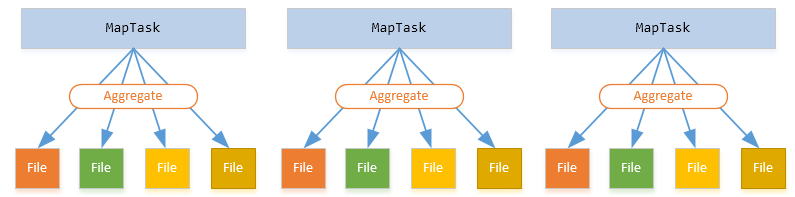
\includegraphics[scale=0.35]{./Figures/spark_shuffle_hash}
  \label{fig:spark_shuffle_hash}
\end{figure}

\begin{itemize}
	\item {\bf Map Tasks write output to multiple files}
	\begin{itemize}
		\item Assume: $m$ map tasks and $r$ reduce tasks
		\item Then: $m \times r$ shuffle files as well as in-memory buffers (for batching writes)
	\end{itemize}

	\item {\bf Be careful on storage space requirements!}
	\begin{itemize}
		\item Buffer size must not be too big with many tasks
		\item Buffer size must not be too small, for otherwise throughput decreases
	\end{itemize}
\end{itemize}
}

%%%%%%%%%%%%%%%%%%%%%%%%%%%%%%%%%%%%%%%%%%%%%%%%%%%%%%%%%%
\frame {\frametitle{The Consolidate Hash Shuffle Mechanism}
%%%%%%%%%%%%%%%%%%%%%%%%%%%%%%%%%%%%%%%%%%%%%%%%%%%%%%%%%%
\begin{figure}[h]
  \centering
  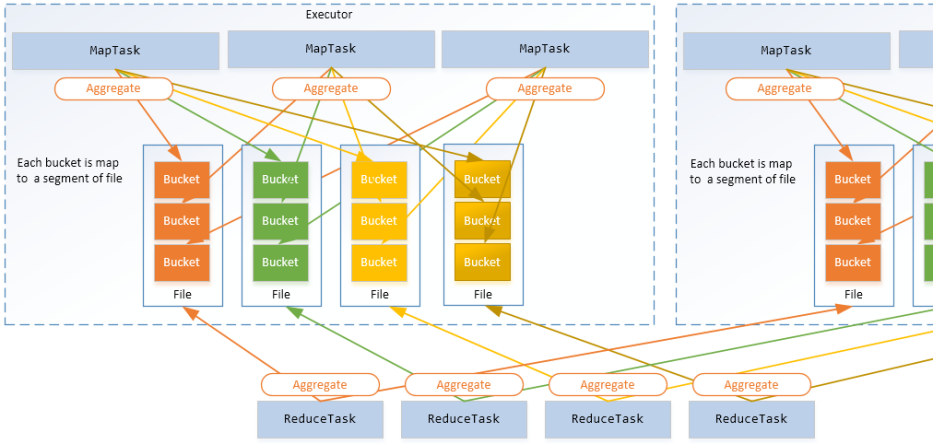
\includegraphics[scale=0.35]{./Figures/spark_shuffle_consolidate}
  \label{fig:spark_shuffle_consolidate}
\end{figure}

\begin{itemize}
	\item {\bf Addresses buffer size problems}
	\begin{itemize}
		\item Executor view vs. Task view
		\item Buckets are consolidated in a single file
		\item Hence: $F = C \times r$ files and buffers, where $C$ is the number of Task threads within an Executor
	\end{itemize}

\end{itemize}
}

%%%%%%%%%%%%%%%%%%%%%%%%%%%%%%%%%%%%%%%%%%%%%%%%%%%%%%%%%%
\frame {\frametitle{The Sort-based Shuffle Mechanism}
%%%%%%%%%%%%%%%%%%%%%%%%%%%%%%%%%%%%%%%%%%%%%%%%%%%%%%%%%%
\begin{figure}[h]
  \centering
  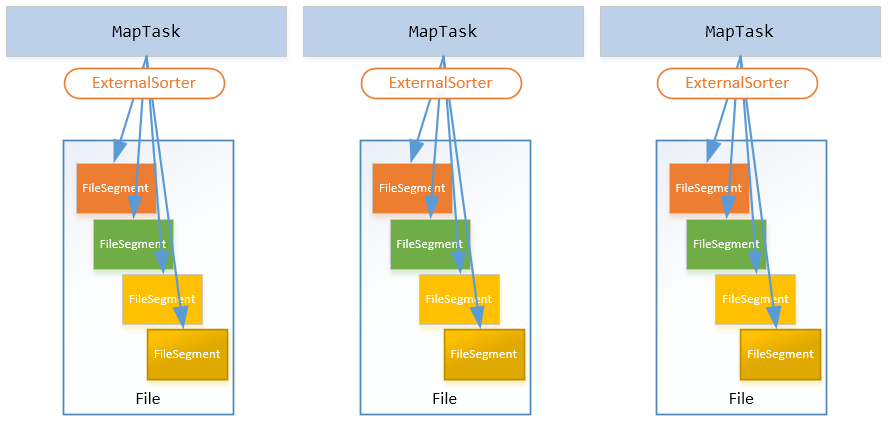
\includegraphics[scale=0.35]{./Figures/spark_shuffle_sort}
  \label{fig:spark_shuffle_sort}
\end{figure}

\begin{itemize}
	\item {\bf Implements the Hadoop Shuffle mechanism}
	\begin{itemize}
		\item Single shuffle file, plus an index file to find ``buckets''
		\item Very beneficial for write throughput, as more disk writes can be batched
	\end{itemize}

	\item {\bf Sorting mechanism}
	\begin{itemize}
		\item Pluggable external sorter
		\item Degenerates to Hash Shuffle if no sorting is required
	\end{itemize}

\end{itemize}
}

%%%%%%%%%%%%%%%%%%%%%%%%%%%%%%%%%%%%%%%%%%%%%%%%%%%%%%%%%%
\frame {\frametitle{Data Transfer: Implementation Details}
%%%%%%%%%%%%%%%%%%%%%%%%%%%%%%%%%%%%%%%%%%%%%%%%%%%%%%%%%%
\begin{itemize}
	\item {\bf BlockTransfer Service}
	\begin{itemize}
		\item General interface for \texttt{ShuffleFetcher}
		\item Uses \texttt{BlockDataManager} to get local data
	\end{itemize}

	\vspace{10pt}

	\item {\bf Shuffle Client}
	\begin{itemize}
		\item Manages and wraps the ``client-side'', setting up the \texttt{TransportContext} and \texttt{TransportClient}
	\end{itemize}
	
	\vspace{10pt}

	\item {\bf Transport Context}: manages the transport layer
	\item {\bf Transport Server}: streaming server
	\item {\bf Transport Client}: fetches consecutive chunks
\end{itemize}
}

%%%%%%%%%%%%%%%%%%%%%%%%%%%%%%%%%%%%%%%%%%%%%%%%%%%%%%%%%%
\frame {\frametitle{Data Transfer: an Illustration}
%%%%%%%%%%%%%%%%%%%%%%%%%%%%%%%%%%%%%%%%%%%%%%%%%%%%%%%%%%
\begin{figure}[h]
  \centering
  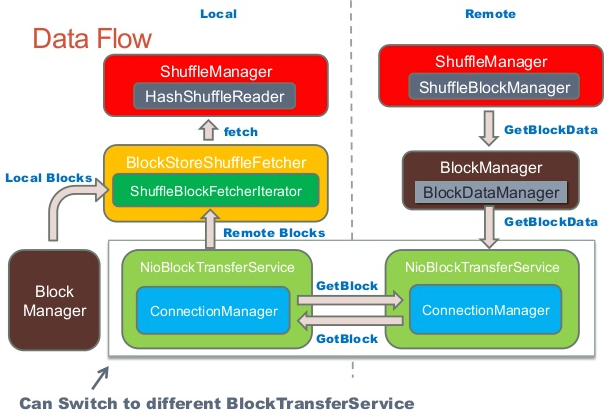
\includegraphics[scale=0.35]{./Figures/shuffle_data_transfer}
  \label{fig:spark_shuffle_sort}
\end{figure}
}
